\documentclass[tikz,border=5pt]{standalone}
\usepackage{helvet}
\renewcommand{\familydefault}{\sfdefault}
\usetikzlibrary{arrows.meta,positioning}

\begin{document}
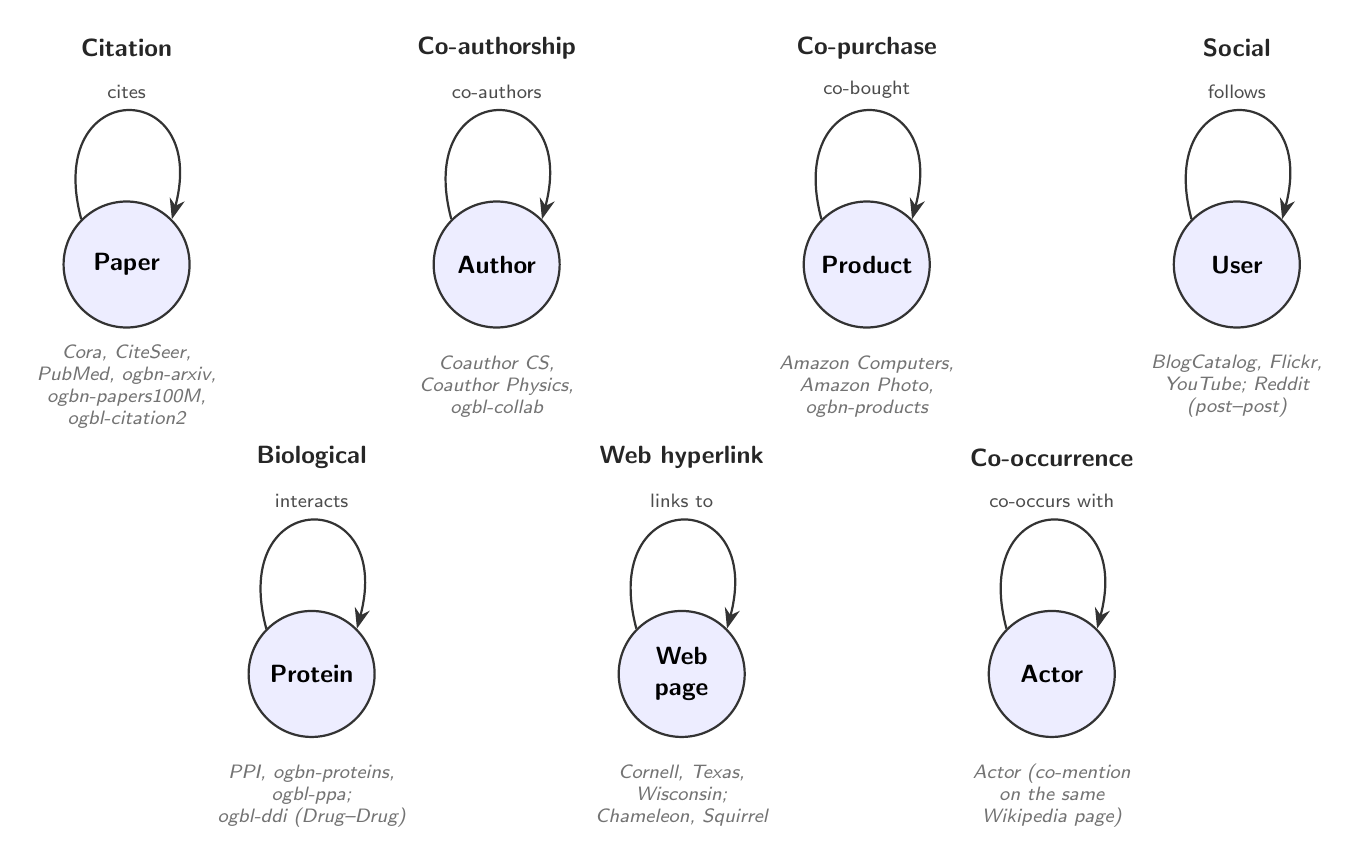
\begin{tikzpicture}[
  font=\small,
  ent/.style={circle, draw=black!80, fill=blue!7, line width=0.8pt,
              minimum size=16mm, inner sep=1pt, align=center,
              font=\small\bfseries},
  rel/.style={-{Stealth[length=2.6mm]}, line width=0.8pt, draw=black!80},
  fam/.style={font=\small\bfseries, align=center, text=black!85},
  note/.style={font=\scriptsize\itshape, text=black!55, align=center},
]

% 4 cells on the top row, 3 centred beneath, so the figure stays wide rather than tall
\def\colA{0}
\def\colB{4.7}
\def\colC{9.4}
\def\colD{14.1}
\def\colE{2.35}
\def\colF{7.05}
\def\colG{11.75}
\def\rowA{0}
\def\rowB{-5.2}

% #1 node-id, #2 x, #3 y, #4 entity, #5 relation, #6 family name, #7 datasets
\newcommand{\schema}[7]{%
  \node[fam] at (#2,{#3+2.75}) {#6};
  \node[ent] (#1) at (#2,#3) {#4};
  % compact self-loop sitting on top of the node: one node type, one edge type
  \draw[rel] (#1.north west) to[out=105,in=75,looseness=4.2]
        node[above=0.4mm, font=\scriptsize, text=black!70] {\textsf{#5}} (#1.north east);
  \node[note] at (#2,{#3-1.55}) {#7};
}

\schema{cit}{\colA}{\rowA}{Paper}{cites}{\textsc{Citation}}%
  {Cora, CiteSeer,\\ PubMed, ogbn-arxiv,\\ ogbn-papers100M,\\ ogbl-citation2}
\schema{coa}{\colB}{\rowA}{Author}{co-authors}{\textsc{Co-authorship}}%
  {Coauthor CS,\\ Coauthor Physics,\\ ogbl-collab}
\schema{cop}{\colC}{\rowA}{Product}{co-bought}{\textsc{Co-purchase}}%
  {Amazon Computers,\\ Amazon Photo,\\ ogbn-products}
\schema{soc}{\colD}{\rowA}{User}{follows}{\textsc{Social}}%
  {BlogCatalog, Flickr,\\ YouTube; Reddit\\ (post--post)}

\schema{bio}{\colE}{\rowB}{Protein}{interacts}{\textsc{Biological}}%
  {PPI, ogbn-proteins,\\ ogbl-ppa;\\ ogbl-ddi (Drug--Drug)}
\schema{web}{\colF}{\rowB}{Web\\page}{links to}{\textsc{Web hyperlink}}%
  {Cornell, Texas,\\ Wisconsin;\\ Chameleon, Squirrel}
\schema{occ}{\colG}{\rowB}{Actor}{co-occurs with}{\textsc{Co-occurrence}}%
  {Actor (co-mention\\ on the same\\ Wikipedia page)}

\end{tikzpicture}
\end{document}
